%% Revised and independently verified version, 16 Aug 2026.
%% Standard IEEE conference layout; no margin or font-size reduction.
\documentclass[conference]{IEEEtran}
\IEEEoverridecommandlockouts

\usepackage{cite}
\usepackage{amsmath,amssymb}
\usepackage{booktabs}
\usepackage{tabularx}
\usepackage{url}
\usepackage{tikz}
\usepackage{pgfplots}
\usepackage{microtype}
\usepackage{balance}
\usepackage[hidelinks]{hyperref}
\pgfplotsset{compat=1.16}

\newif\ifanonymous
\anonymousfalse

\ifanonymous
  \hypersetup{pdftitle={Detecting Purpose-Code Gaming in ISO 20022 Payments: A Synthetic Data-Quality Benchmark},pdfauthor={Anonymous}}
\else
  \hypersetup{pdftitle={Detecting Purpose-Code Gaming in ISO 20022 Payments: A Synthetic Data-Quality Benchmark},pdfauthor={Abhishek Sharma}}
\fi

\begin{document}

\title{Detecting Purpose-Code Gaming in ISO~20022 Payments:\\
A Synthetic Data-Quality Benchmark}

\ifanonymous
\author{\IEEEauthorblockN{Anonymous Author(s)}}
\else
\author{\IEEEauthorblockN{Abhishek Sharma}
\IEEEauthorblockA{\textit{Senior Member, IEEE}\\
Independent Researcher\\
abhishek.sharma@ieee.org}}
\fi

\maketitle

\begin{abstract}
ISO~20022 gives payment controls more structured data, but it also gives
message creators choices about where names, addresses, and purpose information
appear. This paper studies \emph{purpose-code gaming}: deliberate changes
intended to lower a modelled alert probability while preserving the payment's
business meaning. We define eleven manipulations across misfielding, code
substitution, and message-path changes. A seeded generator creates synthetic
pain.001 and pacs.008 records, adds ordinary data-quality defects, and labels
adversarial edits. It enforces field-level constraints, serialises well-formed
XML, and supports XSD validation when schemas are supplied. We also introduce
screening-evasion lift (SEL), which measures how much a manipulation increases
modelled pass-through. Across three 200,000-message runs, the best label-free
detector reaches AUC 0.774 but catches only 9.9\% of manipulated messages at an
exact 1\% alert capacity. A supervised model reaches 0.918 in-distribution,
then falls from 0.815 to 0.366 on unseen misfielding. SEL ranges from 1.33 to
1.78. These results are synthetic and model-relative, but they show where
message-level consistency checks help and where broader transaction context is
needed.
\end{abstract}

\begin{IEEEkeywords}
ISO~20022, payment data quality, purpose codes, sanctions screening,
anti-money laundering, adversarial evaluation, synthetic benchmark
\end{IEEEkeywords}

\section{Introduction}
A payment message is both an instruction and a compliance record. Names,
addresses, amounts, and purpose information may feed sanctions, fraud, and
anti-money-laundering controls. The move to ISO~20022 makes much of that
information easier to parse. In CBPR+, purely unstructured party and agent
addresses cease to be supported from 14 November 2026; town and country must
at least appear in designated fields~\cite{swift2026addr}. CPMI's harmonised
data requirements similarly encourage consistent structured data and
registered codes by end-2027, although CPMI is explicit that the requirements
are guidance rather than a regulatory mandate~\cite{cpmi2026}.

Structure does not remove discretion. A message creator still chooses which
optional fields to populate, which purpose code to declare, how much detail to
place in free text, and sometimes which initiation or routing path is used.
Screening is also selective. Published Swift guidance identifies elements that
normally warrant direct screening and allows other fields to provide context
instead~\cite{swiftgp2021}. Purpose and category-purpose codes may influence
processing or monitoring, yet market-practice guidance notes that these codes
are often misunderstood or placed in the wrong field~\cite{pmpg2024}. An
ordinary data-quality error and a deliberate low-scrutiny choice can therefore
leave similar evidence.

That overlap creates a practical evaluation problem. A detector can look good
by finding malformed records, even though malformed records are mostly benign.
It can also earn a high AUC by learning the edit signatures of one generator,
then fail on a manipulation that was absent from training. The relevant
question is narrower than ``can the model spot unusual data?'' It is whether
deliberate changes remain distinguishable from routine error at an alert
capacity a payment operation could actually use.

This paper makes three contributions. It defines eleven message-level
manipulations and states the capability needed for each. It provides a seeded
synthetic benchmark with a tunable rate of ordinary data-quality errors, five
detector baselines, and a leave-one-family-out test. It also introduces
screening-evasion lift (SEL), which separates the benefit gained by the
adversary from the portion removed by a detector. The detectors are
conventional on purpose; the benchmark, the operational measurement, and the
failure cases are the main contribution. No real payment, customer, or
institution-specific alert data is used.

\section{Background and Design Gap}
\subsection{Fields and control boundaries}
The benchmark covers customer credit transfers at two stages: pain.001 at
initiation and pacs.008 between financial institutions. Relevant content
includes \texttt{Purp/Cd}, \texttt{CtgyPurp/Cd}, party names and postal
addresses, \texttt{UltmtDbtr}, and structured or unstructured remittance
information. Purpose describes the underlying reason for a transaction;
category purpose is a higher-level instruction that may affect processing.
Their exact use is corridor- and institution-specific, which is why the paper
does not assign a universal risk meaning to any ISO code.

The address transition is useful context but not the attack itself. A hybrid
address can retain free-text lines while placing town and country in their
designated fields. That improves machine readability, but it does not guarantee
that the most informative identity or location evidence sits in a field read
by every control. Likewise, a valid purpose code can still be implausible for
the creditor's industry or inconsistent with the remittance narrative. The
benchmark treats these as consistency questions, not schema errors.

Selective screening is unavoidable. Reading every string as a party name
would create an unmanageable false-positive burden, while ignoring contextual
fields loses useful evidence. The tested controls therefore represent three
layers: structural validation, consistency checks within one message, and
comparison with a synthetic transaction history. This layering matters later:
message-level checks can catch contradictions, but they cannot recover context
that has been removed or shifted to a different path.

\subsection{Related benchmarks and adversarial framing}
Synthetic AML datasets usually operate at the transaction or graph level.
AMLworld models realistic transaction networks with laundering labels,
SAML-D supplies a labelled synthetic monitoring dataset, and strategic
simulations allow laundering agents to adapt against a detector
\cite{altman2023,oztas2023,wang2025}. These resources study who pays whom, how
much, and when. They do not encode the internal placement of ISO~20022 fields,
so they cannot express a manipulation whose mechanism is that a name, code, or
narrative appears in a different element. Transaction-purpose classification
addresses enrichment of missing or noisy labels, rather than a label selected
strategically~\cite{busson2023}.

Data-quality research also warns against attributing every performance change
to the learning algorithm. Camacho and Rodr\'iguez-G\'omez show that dataset
variants can move anomaly-detection results more than the model choice itself
\cite{camacho2025}. That finding motivates the explicit defect-rate parameter
$\eta$ in this benchmark. The optimisation follows standard cost-bounded
adversarial classification and test-time evasion~\cite{bruckner2011,biggio2013};
the domain-specific part is the finite set of field and path changes that
preserve the synthetic payment objective. We found no cited benchmark that
combines those message-level operations with a controlled accidental-error
floor. This is a scoped literature observation, not a claim of exhaustive
priority.

\section{Threat Model and Manipulations}
The adversary can construct or amend a payment instruction but does not control
a bank's screening system, sanctions lists, or alert threshold. This covers a
corporate originator, a payment-service provider (PSP), or an insider with
legitimate initiation access. Message-path substitution is a stronger
capability: it applies only to a PSP, bank-side actor, or originator that can
choose among available channels. A typical corporate sender cannot simply
select an interbank message type.

A black-box adversary knows public message guidance and receives only a coarse
accept-or-hold outcome. A grey-box adversary also knows the relative ordering
of the benchmark's purpose-code weights. Neither version observes the exact
threshold or a production rule set. The distinction is methodological: it
lets the evaluation ask whether more knowledge makes the evader harder to
catch, without suggesting that any particular bank exposes those weights.

Let $x$ be an illicit synthetic payment instruction, $m$ an admissible
modification, $c(m)$ its operational cost, and $\pi(x)$ the alert probability
in the published screening abstraction. The evader chooses
\begin{equation}
 m^*=\arg\min_m\{\pi(m(x))+\lambda c(m)\}
 \quad\text{s.t.}\quad V(m(x)),\ |m|\leq k,
 \label{eq:evader}
\end{equation}
where $V$ requires the modified record to pass the benchmark's structural and
business checks and preserve the intended transfer. This is a cost-bounded,
test-time evasion problem~\cite{bruckner2011,biggio2013}. It does \emph{not}
imply that every generated XML instance would be accepted or settled by a
production bank.

\begin{table}[!t]
\caption{The eleven benchmark primitives. The labels describe the synthetic
operation, not a claim about every bank's implementation.}
\label{tab:taxonomy}
\centering
\scriptsize
\begin{tabularx}{\columnwidth}{@{}lX@{}}
\toprule
Family & Primitive operations \\
\midrule
P1 misfielding & P1a move an ultimate-party name to remittance text; P1b
destructure address content; P1c truncate a screened name; P1d omit the
ultimate debtor. \\
P2 code choice & P2a replace purpose; P2b replace category purpose; P2c omit
purpose; P2d create a code--narrative mismatch. \\
P3 structure & P3a use an alternate message path; P3b increase in-message
splitting; P3c insert an intermediary representation. \\
\bottomrule
\end{tabularx}
\end{table}

P1 changes where identity or address evidence appears. P2 leaves the container
intact but changes the declared semantics. P3 changes the message path or
decomposition. These families describe the adversary's action; they do not
predict detectability. A manipulation is easier to detect when it leaves an
internal contradiction, regardless of family.

\section{Benchmark and Method}
\subsection{Synthetic population and edits}
The generator builds debtors and creditors with an industry, home country,
corridor, and pair-specific purpose profile. A benign message samples from
that profile and populates party, address, purpose, and remittance fields.
Pain.001 files are allowed to contain ordinary batches so that multiple
transactions are not a perfect gaming indicator. In the default population,
30\% of benign pain.001 files contain between 2 and 49 transactions.

A fraction $\eta$ receives one ordinary data-quality defect. The default mix
is 35\% purpose content placed in remittance text, 30\% partial address
destructuring, 20\% absent ultimate party, and 15\% absent category purpose.
These proportions are controlled benchmark choices, not measured industry
rates. Their classes follow the types of field-use problems described by
PMPG~\cite{pmpg2024}.

A fraction $\rho$ is then marked illicit for the screening abstraction through
a synthetic combination of party and corridor risk. For each such record, the
evader enumerates beneficial primitive sets up to budget $k$. A perfectly
rational minimum would concentrate on one cheap edit and leave too few samples
for several primitives, so the implementation samples from a softmax over
near-optimal responses. Ground truth records the chosen primitives, the alert
probability before and after the edit, and any accidental defect already
present.

\subsection{Validation features and XML}
Five constraint groups produce detector features. Table~\ref{tab:constraints}
separates local checks from those needing context. C1--C2 are intended to
represent low-cost validation; C3--C4 look for contradictions within a
message; C5 requires pair history. The purpose-history feature reflects the
type of new-code and historical-pattern mismatch described by the Federal
Reserve~\cite{frb2026}.

\begin{table}[!t]
\caption{Constraint groups used by the benchmark.}
\label{tab:constraints}
\centering
\scriptsize
\begin{tabularx}{\columnwidth}{@{}lXl@{}}
\toprule
ID & Check & Context \\
\midrule
C1 & Purpose-code membership & field \\
C2 & Required structure and address tokens in free text & message \\
C3 & Purpose--industry, batch, and ultimate-party plausibility & message \\
C4 & Purpose code versus remittance narrative & message \\
C5 & Pair-level purpose distribution versus prior history & history \\
\bottomrule
\end{tabularx}
\end{table}

The field-level records can be serialised as pain.001.001.09 or
pacs.008.001.08. The release checks XML well-formedness and exposes an optional
XSD-validation hook when schemas are supplied. No XSD-validation outcome is
used as experimental evidence, and the paper therefore does not claim that all
emitted instances are production-valid. This distinction also avoids
conflating an XSD pass with channel rules, business validation, or settlement.

\subsection{Screening abstraction and calibration}
The incumbent alert model is transparent rather than institution-specific. A
name leg operates over a stated set of party fields. A score leg combines
purpose, corridor, amount, and completeness, followed by a logistic threshold.
A residual floor represents controls outside the evader's reach. The combined
probability is
\begin{equation}
 \pi(x)=1-(1-p_{\mathrm{name}})(1-p_{\mathrm{score}})(1-f).
 \label{eq:screening}
\end{equation}
The weights are illustrative and published with the code. They are not
estimates of any bank's rule set.

Calibration deserves explicit treatment because P1 mainly attacks the name
leg and P2 mainly attacks the score leg. Setting the desired baseline alert
probability $\pi_0$ by adjusting only one leg can make the other family
irrelevant. The benchmark instead divides baseline survival multiplicatively
between the two legs using a stated name-share parameter $\sigma$. The main
setting uses $\pi_0=0.45$ and $\sigma=0.6$; a $3\times3$ grid varies
$\pi_0\in\{0.30,0.45,0.60\}$ and $\sigma\in\{0.4,0.6,0.8\}$.

\subsection{Detectors and evasion metrics}
$D_0$ applies C1--C2 checks. $D_1$ adds fixed C3--C4 rules. $D_2$ is a
supervised gradient-boosted model over one-hot codes, corridor, amount, and
completeness features. $D_3$ is an isolation forest fitted to benign C1--C5
features~\cite{liu2008}. $D_4$ sums standardised $D_1$ and $D_3$ scores. Only
$D_2$ trains on gaming labels.

AUC measures ranking but not the value of an attack. Let $\pi_0$ be the alert
probability before manipulation and $\pi_m$ after it. We define
\begin{equation}
 \mathrm{SEL}(m)=\frac{1-\pi_m}{1-\pi_0}.
 \label{eq:sel}
\end{equation}
If detector $D$ alerts manipulated and unmanipulated illicit payments at rates
$\delta_m$ and $\delta_0$, the residual lift is
\begin{equation}
 \mathrm{SEL}_{\mathrm{res}}(m,D)=
 \frac{(1-\pi_m)(1-\delta_m)}{(1-\pi_0)(1-\delta_0)}.
 \label{eq:selres}
\end{equation}
SEL of 1 means that the edit provides no modelled benefit. The gap between
SEL and residual SEL is the portion removed by the detector.

\subsection{Evaluation protocol}
The main setting uses 200,000 records per seed, seeds 7--9, $\eta=0.15$,
$\rho=0.05$, $k=2$, $\lambda=0.18$, softmax temperature 0.10, residual floor
0.10, target $\pi_0=0.45$, and a 0.6 name-leg share. We report AUC and true
positive rate at alert capacities of 1\% and 0.1\%.

Discrete detector scores create ties. A plain ``score above quantile'' rule can
therefore alert far more records than the stated capacity. The implementation
selects every score above the boundary and assigns the tied block the
label-blind fraction needed to fill the capacity exactly. At 1\% of 200,000
records this is 2,000 expected alerts, not all records tied with the 2,000th.
Reported TPR is the expectation under uniform tie-breaking.

For generalisation, $D_2$ is retrained while one primitive family is withheld.
The evaluation uses $k=1$ and pure-family messages, preventing a held-out
family from leaking through a second primitive. Its held-out AUC is compared
with an in-distribution AUC on the same rows. The protocol also varies $\eta$,
$k$, adversary knowledge, and the calibration of $\pi$. Configuration, seeds,
and raw JSON outputs are retained with the release.

\section{Results}
\begin{table}[!t]
\caption{Detection results. Panel (a) is the mean of three 200,000-record runs.
TPR is evaluated at an exact alert capacity with label-blind tie-breaking.
Panel (b) uses pure-family records at $k=1$; only $D_2$ is retrained.}
\label{tab:results}
\centering
\scriptsize
\textit{(a) Main setting}\\[-2pt]
\begin{tabular}{@{}lcccc@{}}
\toprule
Detector & Labels & AUC & TPR@1\% & TPR@0.1\% \\
\midrule
$D_0$ C1--C2 checks & no & 0.497 & 0.009 & 0.001 \\
$D_1$ fixed rules & no & 0.750 & 0.105 & 0.020 \\
$D_2$ supervised & yes & \textbf{0.918} & \textbf{0.201} & \textbf{0.020} \\
$D_3$ anomaly & no & 0.752 & 0.040 & 0.007 \\
$D_4$ combined & no & 0.774 & 0.099 & 0.018 \\
\bottomrule
\end{tabular}

\vspace{3pt}
\textit{(b) Leave-one-family-out}\\[-2pt]
\begin{tabular}{@{}lcccc@{}}
\toprule
Family & $n$ & $D_1$ & $D_2$: in $\rightarrow$ out & $D_4$ \\
\midrule
P1 misfielding & 3980 & 0.733 & 0.815 $\rightarrow$ \textbf{0.366} & 0.744 \\
P2 code choice & 1728 & 0.843 & 0.989 $\rightarrow$ 0.779 & 0.800 \\
P3 structure & 3917 & 0.445 & 0.689 $\rightarrow$ 0.487 & 0.484 \\
\bottomrule
\end{tabular}
\end{table}

Table~\ref{tab:results}(a) shows a large gap between ranking and useful
recovery. $D_4$ separates manipulated from ordinary records with AUC 0.774,
yet it finds only 9.9\% of manipulations when exactly 1\% of all records may be
alerted. At 0.1\% capacity, recovery is 1.8\%. The supervised $D_2$ reaches
AUC 0.918 and doubles the 1\% recovery, but it assumes labels that are unlikely
to exist for new manipulations.

Table~\ref{tab:results}(b) shows how brittle that supervised advantage can be.
When P1 is absent from training, $D_2$ falls from 0.815 to 0.366 on the same
evaluation rows. Its P2 drop is smaller but still material. P3 is not usefully
separated by the tested message-level controls: $D_4$ scores 0.484 in the
pure-family test and $D_1$ scores 0.445. These numbers do not establish that P3
is inherently hidden. They show that the current fields and features provide
little direction for ranking it.

\begin{figure}[!t]
\centering
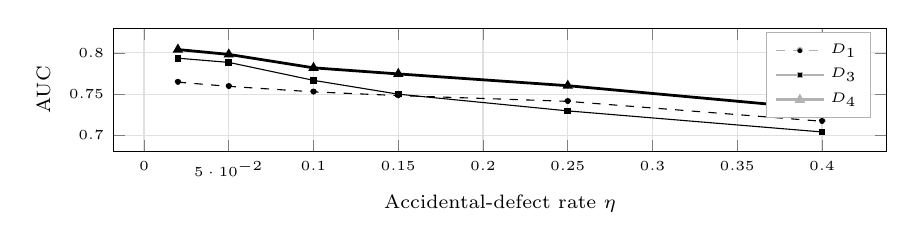
\begin{tikzpicture}
\begin{axis}[
  width=0.94\columnwidth,height=3.15cm,
  xlabel={Accidental-defect rate $\eta$},ylabel={AUC},
  ymin=0.68,ymax=0.83,grid=both,grid style={black!12},
  legend style={at={(0.98,0.97)},anchor=north east,font=\tiny,draw=black!30},
  label style={font=\scriptsize},tick label style={font=\tiny}
]
\addplot[dashed,mark=*,mark size=1pt] coordinates {(0.02,0.7645) (0.05,0.7594) (0.10,0.7527) (0.15,0.7482) (0.25,0.7412) (0.40,0.7170)};
\addlegendentry{$D_1$}
\addplot[solid,mark=square*,mark size=1pt] coordinates {(0.02,0.7936) (0.05,0.7885) (0.10,0.7667) (0.15,0.7499) (0.25,0.7296) (0.40,0.7040)};
\addlegendentry{$D_3$}
\addplot[solid,line width=1.0pt,mark=triangle*,mark size=1.2pt] coordinates {(0.02,0.8041) (0.05,0.7982) (0.10,0.7819) (0.15,0.7745) (0.25,0.7602) (0.40,0.7319)};
\addlegendentry{$D_4$}
\end{axis}
\end{tikzpicture}
\caption{AUC as the ordinary defect rate rises. Each point uses 100,000
records at seed 7; only AUC, which is unaffected by threshold ties, is shown.}
\label{fig:eta}
\end{figure}

The noise experiment in Fig.~\ref{fig:eta} shows gradual degradation rather
than collapse. Raising $\eta$ from 0.02 to 0.40 lowers $D_4$ AUC by 0.072. The
fixed rules are the most stable. The anomaly model degrades faster because the
benign distribution it learns is itself moving. At the highest noise rate,
$D_1$ and $D_4$ still rank above chance, but the main operational result warns
against treating that ranking as sufficient.

\begin{figure}[!t]
\centering
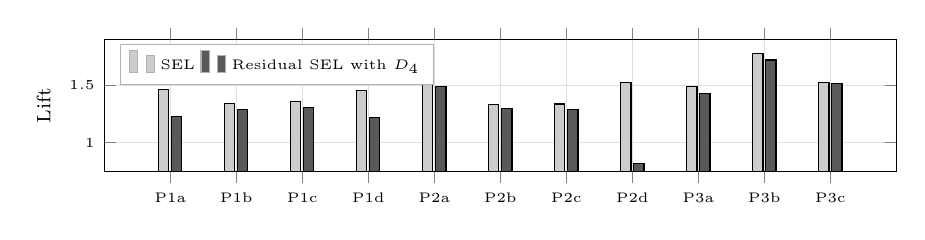
\begin{tikzpicture}
\begin{axis}[
  width=0.96\columnwidth,height=3.25cm,
  ybar=1pt,bar width=3.7pt,ylabel={Lift},
  symbolic x coords={P1a,P1b,P1c,P1d,P2a,P2b,P2c,P2d,P3a,P3b,P3c},
  xtick=data,ymin=0.75,ymax=1.9,grid=both,grid style={black!12},
  legend style={at={(0.02,0.97)},anchor=north west,font=\tiny,draw=black!30,legend columns=2},
  label style={font=\scriptsize},tick label style={font=\tiny}
]
\addplot[fill=black!20] coordinates {(P1a,1.464) (P1b,1.341) (P1c,1.362) (P1d,1.456) (P2a,1.522) (P2b,1.334) (P2c,1.338) (P2d,1.525) (P3a,1.493) (P3b,1.777) (P3c,1.526)};
\addlegendentry{SEL}
\addplot[fill=black!65] coordinates {(P1a,1.225) (P1b,1.287) (P1c,1.310) (P1d,1.222) (P2a,1.487) (P2b,1.297) (P2c,1.289) (P2d,0.817) (P3a,1.431) (P3b,1.723) (P3c,1.517)};
\addlegendentry{Residual SEL with $D_4$}
\end{axis}
\end{tikzpicture}
\caption{Mean screening-evasion lift before and after $D_4$ across three
seeds. Values are relative to the published screening abstraction.}
\label{fig:sel}
\end{figure}

Manipulation increases modelled pass-through by 33\%--78\% in the main
calibration. The detector's value varies sharply by primitive. For the
code--narrative mismatch P2d, residual lift falls below 1
($1.525\rightarrow0.817$), so the added check more than removes the simulated
benefit. For in-message splitting P3b, it barely changes
($1.777\rightarrow1.723$). P3c is even more stark in detection rate: only about
0.6\% of its selected instances are alerted by $D_4$ at the 1\% capacity.
Residual SEL should nevertheless be read cautiously because the unevaded
illicit baseline contains only 57--60 records per seed in this configuration.

Across the $3\times3$ calibration grid, SEL ranges from 1.13 to 2.59 while
$D_4$ AUC remains between 0.772 and 0.795. The size of the modelled threat is
therefore sensitive to the assumed baseline and name-share, while the relative
detection difficulty is more stable. This is why the release reports the grid
rather than treating one SEL number as a deployment estimate.

\begin{table}[!t]
\caption{$D_4$ ablations, 100,000 records at seed 7 per setting.}
\label{tab:ablations}
\centering
\scriptsize
\begin{tabular}{@{}llc@{}}
\toprule
Factor & Setting & AUC \\
\midrule
Primitive family & P1 / P2 / P3 & 0.794 / 0.834 / 0.548 \\
Evader budget & $k=1$ / $k=2$ / $k=3$ & 0.647 / 0.774 / 0.844 \\
Knowledge & black / grey & 0.738 / 0.774 \\
\bottomrule
\end{tabular}
\end{table}

Table~\ref{tab:ablations} supports the same interpretation. More edits make the
evader easier to rank because each edit can leave another inconsistency. The
grey-box adversary is also easier to detect than the black-box one: acting on
code-weight knowledge touches fields that C3--C4 examine. A more informed
adversary is therefore not automatically a stealthier one in this benchmark.

\section{Discussion and Limitations}
The practical lesson is not that structured data weakens controls. It gives
controls better inputs and enables useful consistency checks. The narrower
lesson is that validation, screening coverage, and behavioural monitoring must
be designed together. C1--C2 catch malformed or incomplete data. C3--C4 catch
contradictions within one message. C5 or other longitudinal features are
needed when the message is internally plausible. Changes to path, batch
structure, or party chain may require channel history, agent-chain context, or
comparison with the originator's normal files. A message-only model cannot
infer evidence that the message does not contain.

The study also separates detector credit from incumbent-control credit. A
primitive can be easy to classify yet offer little extra protection if the
incumbent model would already alert it. Conversely, modest AUC can still be
useful for a narrow primitive if it removes substantial lift at the operating
threshold. SEL and residual SEL make that distinction visible, but they inherit
the assumptions of $\pi$.

Several limitations remain. The screening abstraction is transparent and
reproducible, not a reconstruction of a bank's engine, so SEL is a stress
measure rather than an estimate of losses or real evasion. The distributions
of purpose codes, defects, batching, and illicit traffic are assumptions. The
generator and detectors also share a feature vocabulary, which can reward
recognition of implementation artefacts; the leave-one-family-out collapse of
$D_2$ demonstrates the risk rather than solving it. External validity requires
recalibration on an institution's own traffic.

The XML layer has a similarly narrow claim. The serializers are checked for
well-formedness, the pain.001 ultimate-debtor ordering was corrected during
review, and the harness accepts external XSDs. The release does not treat XSD
validity as proof of business acceptance. P3a is also capability-dependent and
should not be attributed to an ordinary corporate originator without route
choice.

The corpus uses synthetic entities and illustrative weights. It contains no
customer records, employer data, production alert outcomes, or corridor-tuned
control parameters. The primitive taxonomy is published for defensive coverage
analysis: an institution can map the families to its own screened fields,
message paths, and history features without disclosing payment data. A stronger
next experiment would calibrate $\pi$ against anonymised alert outcomes inside
one institution and evaluate path-aware controls without exporting raw
messages.

\section{Conclusion}
Purpose-code gaming remains distinguishable from routine data-quality error in
this benchmark, but good AUC does not translate into strong recovery at a small
alert capacity. Message-level checks work best when an edit creates a
contradiction, as P2d does, and poorly when the edit changes the container while
remaining internally coherent. The supervised model's failure on an unseen
family reinforces the same point: recognition of known edit signatures is not
the same as coverage of the underlying risk. The release provides a compact
way to test that boundary, together with the assumptions needed to challenge
it.


\balance
\begin{thebibliography}{99}
\scriptsize
\setlength{\itemsep}{0pt plus 0.2pt}

\bibitem{swift2026addr}
Swift, ``ISO~20022: The removal of unstructured address,'' Swift Standards,
2026. [Online]. Available:
\url{https://www.swift.com/standards/iso-20022/iso-20022-faqs/iso-20022-removal-unstructured-address}

\bibitem{cpmi2026}
Committee on Payments and Market Infrastructures, \emph{Harmonised ISO~20022
Data Requirements for Enhancing Cross-Border Payments}, Bank for International
Settlements, updated report, Feb. 2026.

\bibitem{swiftgp2021}
Swift, \emph{Guiding Principles for Screening ISO~20022 Payments Messages},
Oct. 2021.

\bibitem{pmpg2024}
Payments Market Practice Group, \emph{ISO~20022 Market Practice Guidance:
Regulatory Reporting, Purpose of Payment and Category Purpose}, ver. 1.1, Jul.
2024.

\bibitem{altman2023}
E. Altman \emph{et al.}, ``Realistic synthetic financial transactions for
anti-money laundering models,'' in \emph{Advances in Neural Information
Processing Systems}, vol. 36, 2023.

\bibitem{oztas2023}
B. Oztas \emph{et al.}, ``Enhancing anti-money laundering: Development of a
synthetic transaction monitoring dataset,'' in \emph{Proc. IEEE ICEBE}, 2023,
pp. 47--54.

\bibitem{wang2025}
Q. Wang, W.-T. Tsai, T. Shi, W. Tang, and B. Du, ``Hide and seek in
transaction networks: A multi-agent framework for simulating and detecting
money laundering activities,'' \emph{Complex \& Intelligent Systems}, vol. 11,
art. 271, 2025.

\bibitem{busson2023}
A. J. G. Busson \emph{et al.}, ``Hierarchical classification of financial
transactions through context-fusion of transformer-based embeddings and
taxonomy-aware attention layer,'' arXiv:2312.07730, 2023.

\bibitem{camacho2025}
J. Camacho and R. A. Rodr\'iguez-G\'omez, ``Data quality tools to enhance a
network anomaly detection benchmark,'' \emph{Data}, vol. 10, no. 3, art. 33,
2025.

\bibitem{bruckner2011}
M. Br\"uckner and T. Scheffer, ``Stackelberg games for adversarial prediction
problems,'' in \emph{Proc. ACM SIGKDD}, 2011, pp. 547--555.

\bibitem{biggio2013}
B. Biggio \emph{et al.}, ``Evasion attacks against machine learning at test
time,'' in \emph{Proc. ECML PKDD}, 2013, pp. 387--402.

\bibitem{frb2026}
Federal Reserve Financial Services, ``Harnessing the power of ISO~20022: Why
the global payment standard matters for fraud mitigation,'' \emph{Fed360}, 15
Apr. 2026.

\bibitem{liu2008}
F. T. Liu, K. M. Ting, and Z.-H. Zhou, ``Isolation forest,'' in \emph{Proc.
IEEE ICDM}, 2008, pp. 413--422.

\end{thebibliography}

\end{document}
